\newpage
\section{Einführung}
Die \textbf{Frequenzmodulationssynthese} ist eine für die Musikwelt sehr wichtige Anwendung der \textbf{Frequenzmodulation (FM)}, welche bereits aus der Nachrichtentechnik bekannt ist. Eine Motivation für diese Seminararbeit ist die Tatsache, dass die Musikwelt durch FM-Synthese eine Revolution erlebt hat und ohne diese Erfindung eine Vielzahl an Synthesizern niemals entstanden wäre. Die Arbeit ist im Rahmen des Vertiefungsseminars I der Vertiefung Medieninformatik an der Hochschule für angewandte Wissenschaften Würzburg-Schweinfurt entstanden. %WIP, wer bock hat mag sich was besseres ausdenken :D
\FloatBarrier
\subsection{Prinzip der FM-Synthese}
\label{PrinzipFM}
Generell wird bei der Frequenzmodulation die Frequenz eines \textbf{Trägersignals} durch ein weiteres \textbf{Modulationssignal} verändert, die Amplitude bleibt jedoch unangetastet. In der Nachrichtentechnik können durch die unterschiedlichen Frequenzen im modulierten Träger Informationen übertragen werden. Bei der FM-Synthese kann die maximale Amplitude in besonderen Fällen jedoch von der maximalen Auslenkung des Trägers abweichen bzw. kleiner als diese werden. 
Die momentane Amplitude der Modulation lässt sich bei der FM-Synthese durch folgende Formel beschreiben:
\begin{equation}
e(t) = A\sin(\alpha t + I\sin(\beta t)) \cite{chowningPaper}
\end{equation}
Bei der äußeren Sinusfunktion handelt es sich um den Träger, welcher in seiner Frequenz durch das Modulationssignal (innerer Sinus) moduliert wird. \textbf{Abbildung \ref{fig:vergleichSignale}} veranschaulicht die Frequenzmodulation eines Trägers durch den Modulator.

\begin{figure} [ht]
\centering
  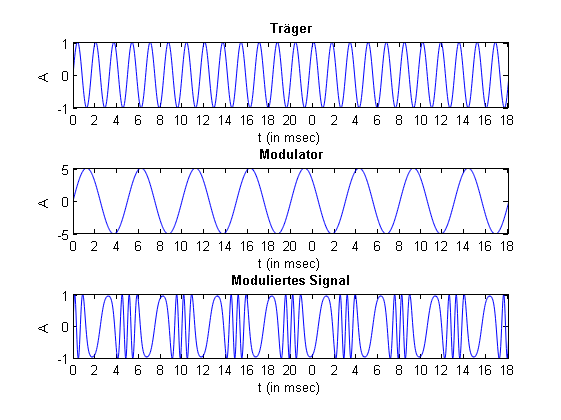
\includegraphics[width=0.95\textwidth]{Prinzip.png}
\caption{Vergleich Träger/Modulator}
\label{fig:vergleichSignale}
\end{figure}
\FloatBarrier

Technisch gesehen kann die FM-Synthese mit Oszillatoren umgesetzt werden. In der einfachsten Form benötigt man dazu einen Träger-Oszillator und einen Modulator-Oszillator. Wie eine einfache FM-Synthese in Form einer Schaltung aussehen kann, zeigt \textbf{Abbildung \ref{fig:schaltung}}. Der Ausgang des ersten Oszillators geht dabei in den Eingang des Zweiten. Dabei kann entweder direkt die Frequenz des Trägers beeinflusst werden, jedoch auch dessen Phase. Bei VCA handelt es sich um einen spannungsgesteuerten Verstärker (Voltage Controlled Amplifier), EG ist ein Hüllkurvengenerator (Envelope Generator). Bei den Parametern $f_M$ und $f_C$ handelt es sich um die Frequenzen der beiden Oszillatoren. Über den Modulationsindex $\beta$ kann die Stärke der Modulation festgelegt werden. 

\begin{figure} [ht]
\centering
  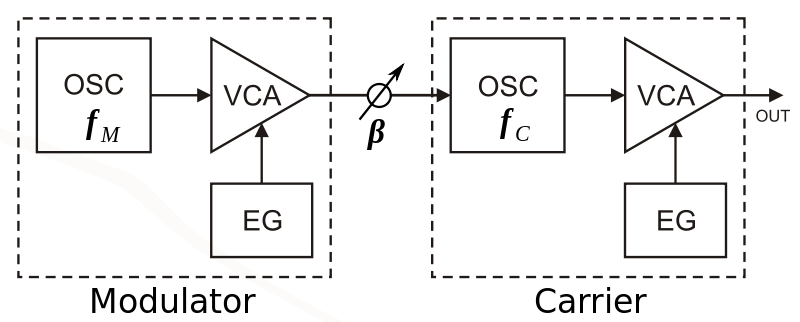
\includegraphics[width=0.8\textwidth,frame]{schaltung.png}
\caption{Schaltung einer einfachen FM-Synthese}
\label{fig:schaltung}
Quelle: \url{http://mmmmaven.com/wp-content/uploads/800px-2op_FM.svg_.png} 
\\Stand 16.06.2015
\end{figure}

Die Frequenzmodulationssynthese ist in ihren Grundzügen recht einfach zu verstehen. Es können mit geringem Aufwand bereits sehr komplexe, wenn auch oft unkontrollierbare, Signale mit komplexen Klangspektren (bzw. Frequenzspektren) erzeugt werden. Wie sich im Folgenden jedoch noch herausstellen wird, ist es dagegen sehr schwierig, durch die FM-Synthese gezielt Signale zu formen und diese zu kontrollieren.

Praktisch gesehen kann die Frequenzmodulationssynthese dazu verwendet werden, Klangbilder echter Instrumente nachzubilden, jedoch auch für die Erzeugung ganz neuer Töne, die so nicht in der Natur vorkommen.

\FloatBarrier
\subsection{Beispiele}
In diesem Kapitel werden einige konkrete Beispiele der FM-Synthese anhand von Träger- und Modulationssignal sowie des daraus resultierenden Signals aufgezeigt. Die Grafiken zeigen jeweils Plots von allen drei Signalen, welche in MATLAB erzeugt wurden.
Die Frequenzen der jeweiligen Funktionen wurden so gewählt, dass sie in einem Frequenzbereich liegen, der vom menschlichen Ohr wahrgenommen werden kann (siehe \textbf{``\ref{bulli:ohrToeneUndFrequenzen} - \nameref{bulli:ohrToeneUndFrequenzen}''}).

\begin{figure} [ht]
\centering
  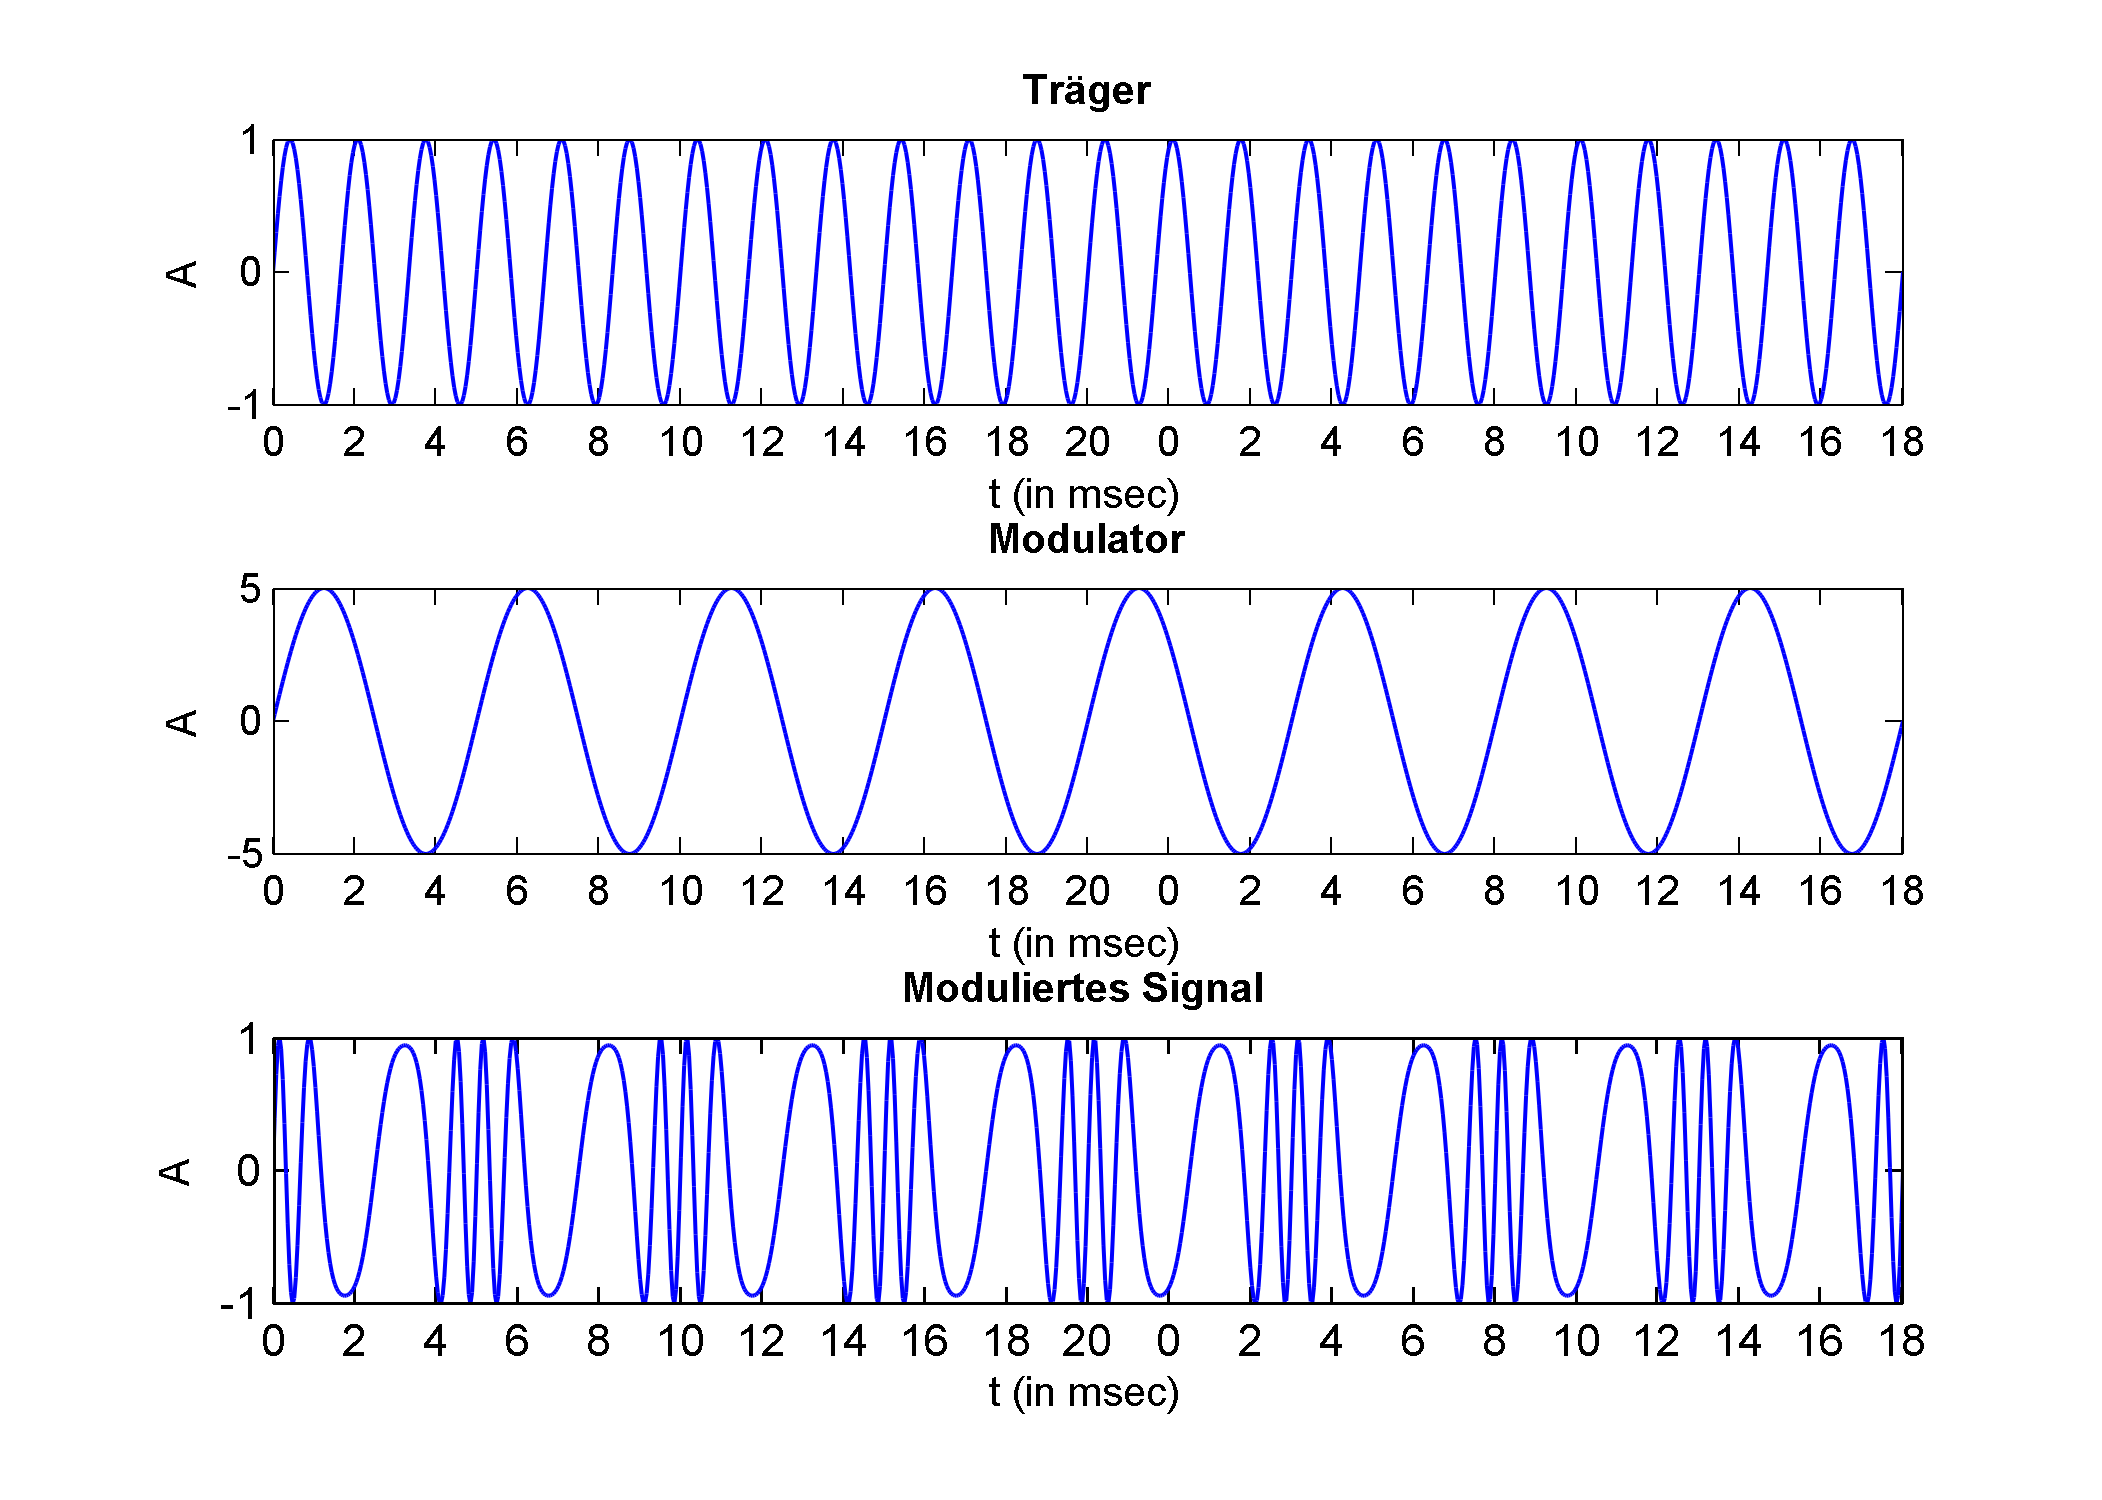
\includegraphics[width=0.95\textwidth]{Beispiel1.png}
\caption{Beispiel 1. Darstellung einer Frequenzmodulation mit einer Trägerfrequenz von 600 Hz, einer Modulationsfrequenz von 75 Hz und einem Modulationsindex von 5 }
\label{fig:beispiel1}
\end{figure}

In Beispiel 1 (siehe \textbf{Abbildung \ref{fig:beispiel1}})  wurden folgende Signale verwendet:

\begin{lstlisting}[mathescape]
Trägersignal: 		$y(t) \;=\; \,\;\;\sin(2 \pi 600\cdot t)$
Modulator:		$y(t) \;=\; 5 \sin(2 \pi 75 \;\; \cdot t)$
Gesamtfunktion: 	$y(t) \;=\; \,\;\;\sin(2 \pi 600\cdot t + 5 \sin(2 \pi 75\cdot t))$
\end{lstlisting}


Konkret bedeuted eine Trägerfrequenz von 600 Hz, dass die Trägerfunktion 600 mal in der Sekunde schwingt, d.h. eine Periode ist genau $\frac{1}{600}$ Sekunden lang. Der Modulator hat eine Frequenz von 75 Hz, wodurch er 75 Schwingung pro Sekunde durchläuft und eine Periode dann $\frac{1}{75}$ Sekunden lang ist. Für die Modulation gilt im Allgemeinen, dass der sogenannte Frequenzhub der Modulation (siehe Kapitel \textbf{``\ref{chowningparameter} - \nameref{chowningparameter}''}) immer dann maximal ist, wenn die Änderung der Modulationsfunktion (also deren Steigung) ihr Maximum bzw. Minimum hat. In der Grafik tritt dies immer dann auf, wenn der Modulator den Funktionswert 0 hat.

\begin{figure} [ht]
\centering
  \includegraphics[width=0.95\textwidth]{Beispiel2.png}
\caption{Beispiel 2. Darstellung einer Frequenzmodulation mit einer Trägerfrequenz von 300 Hz, einer Modulationsfrequenz von 120 Hz und einem Modulationsindex von 5}
\label{fig:beispiel2}
\end{figure}

Das zweite Beispiel in \textbf{Abbildung \ref{fig:beispiel2}} zeigt eine Frequenzmodulation, bei der sich auch die Amplitude des Signals ändert. Dies geschieht rein durch die Phasenverschiebung des äußeren Sinus durch den Modulator, die tatsächliche Amplitude der Funktion bleibt dabei unangetastet. Die Formel des modulierten Signals sieht wie folgt aus:

\begin{equation}
y(t) = \sin(2 \pi 300\cdot t + 5 \sin(2 \pi 120\cdot t))
\end{equation}

An diesem Beispiel kann man sehr gut erkennen, dass die FM-Synthese mit wenig Aufwand komplexe Signale erzeugen kann, diese jedoch schlecht kontrollierbar bzw. erklärbar sind.

Als gute akustische Beispiele für die Anwendung der FM-Synthese in der Musikwelt können die Stücke \textbf{``Sabelith''} und \textbf{``Turenas'}' von John Chowning, dem Erfinder der FM-Synthese, genannt werden. Beide Stücke wurden ausschließlich mit den Mitteln der FM-Synthese erzeugt und beinhalten viele verschiedene Klangarten sowie synthetisierte Instrumente.

\FloatBarrier
\subsection{Geschichte der FM-Synthese}
\label{geschichteFMSynthese}
Die grundlegende Technik hinter der FM-Synthese stammt, wie bereits erwähnt, aus der Nachrichtentechnik. Dort wird das Verfahren ``Frequenzmodulation'' genannt. Prof. Dr. John Chowning selbst gibt als Quelle zu seiner Entdeckung das Buch ``Radio Engineering'' von Frederick Emmons Terman aus dem Jahre 1947 an \cite[S. 35]{soundofinnovation}. Im Jahr 1967 entdeckte John Chowning eine neue Eigenschaft der Frequenzmodulation. Während er mit unterschiedlichen Modulationsfrequenzen experimentierte und dabei verschiedene Vibratos erzeugte, verschwand das Vibrato plötzlich bei höheren Modulationsfrequenzen. Obertöne wurden hörbar, die sich vom eigentlichen Trägersignal abhebten. Unter einem Vibrato versteht man einen schwingenden Ton, d.h. eine pulsierende Änderung der Tonhöhe.\cite{fatherofdigitalmusik}

Chowning selbst war sehr erstaunt über die entstandenen Töne. In einem Interview von 2005 sagte er dazu: 

\textit{``I was experimenting with just a sinusoid and kept increasing the vibrato rate, so all of a sudden it didn't sound like listening to a change in pitch in time, but rather i began to hear timbral differences. So the vibratio became very, very fast, hundreds of times per second, and very, very deep, as if the violinist had a different fingerboard, and the finger was whipping up and down at very high rates and very great distances. That would be sort of a physical metaphor for this.''}\cite[S. 34f.]{soundofinnovation}

Es dauerte 3 Jahre, bis sich Chowning seiner Sache gewiss war und die mathematischen Zusammenhänge ausreichend begründen konnte. Außerdem war er zu diesem Zeitpunkt bereits in der Lage, verschiedene Instrumente wie Trommeln oder Blasinstrumente nachzubilden. Da Chowning selbst leidenschaftlicher Komponist war, veröffentlichte er im Jahre 1971 sein erstes, rein durch FM-Synthese generiertes Stück mit dem Namen ``Sabelithe''. Seine zweite Komposition, ``Turenas'', folgte ein Jahr später.
Um die Stärken seiner neuen Technik zu demonstrieren, verwandelte Chowning beispielsweise in ``Sabelithe'' den Klang einer Trommel in den einer Trompete.\cite[S. 39]{soundofinnovation}
 
\begin{figure} [ht]
\centering
  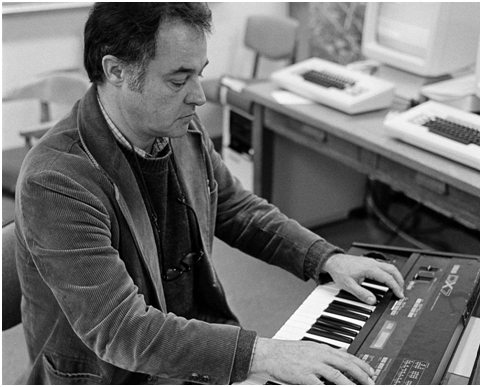
\includegraphics[width=0.8\textwidth]{chowning_CCRMA.png}
\caption{John Chowning am CCRMA}
\label{fig:chowningdx7}
Quelle: \url{ http://arts.mit.edu/wp-content/uploads/2014/07/ChowningYamaha.jpg} \\Stand 09.06.2015
\end{figure}
 
Chowning war, wie auch seine Kollegen, eher Komponist als Erfinder. Aus diesem Grund waren sie eher an der musikalischen Seite der Erfindung interessiert als an kommerziellem Erfolg. Obwohl er das Potenzial seiner Erfindung zu dieser Zeit noch nicht überblicken konnte, wendete sich Chowning an das OTL (Office of Technology Licensing) in Stanford. Er hoffte, dass es in der Musikindustrie eine sinnvolle Anwendung seiner Entdeckung gab.\cite[S. 42]{soundofinnovation}

 Zu Beginn war seine Entdeckung jedoch nicht sehr angesehen. Viele der Firmen, welchen das neue Patent angeboten wurde, wussten nichts damit anzufangen und lehnten ab. Andy Moorer, ein Kollege Chownings in Stanford und später Mitgründer des CCRMA, sagte dazu: 

\textit{``[...] It was really discouraging. John was so proud of having put this damn thing together and people didn't really get the idea of spatializing the sound.''}\cite[S. 43]{soundofinnovation}

Offiziell veröffentlichte John Chowning seine neue Entdeckung der Frequenzmodulationssynthese in einem Paper, welches 1973 im ``Journal of the Audio Engineering Society'' unter dem Titel ``The Synthesis of Complex Audio Spectra by Means of Frequenzy Modulation'' erschien.

Erst im Jahr 1974, als ein junger Ingenieur namens Kazukiyo Ishimura der Firma Yamaha zu einer Vorstellung des Verfahrens geschickt wurde, erkannte dieser binnen wenigen Minuten, welches Potenzial hinter dieser neuen Anwendung der Frequenzmodulation steckt. Yamaha lizensierte das Verfahren noch im gleichen Jahr und Ishimura wurde später Geschäftsführer des Yamaha Konzerns \cite{fatherofdigitalmusik}.

Im Jahr 1975, nach einiger Zeit der Abwesenheit von Stanford, kehrte Chowning dorthin zurück und gründete zusammen mit einigen seiner Kollegen das CCRMA (Center for Computer Research in Music and Acoustics), welches sich auf computergenerierte Musik spezialisiert hat.
Eine Fotografie der Gründer von CCRMA ist auf \textbf{Abbildung \ref{fig:foundersCCRMA}} zu sehen.

\begin{figure} [ht]
\centering
  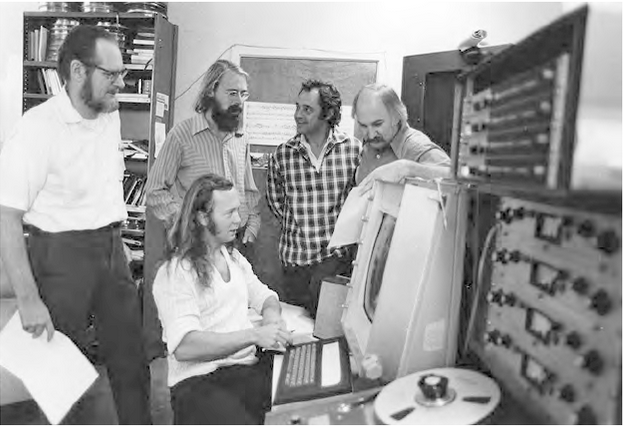
\includegraphics[width=0.8\textwidth]{Founders_CCRMA.png}
\caption{Gründer von CCRMA. Stehend von links nach rechts: Leland Smith, John Grea, John Chowning und Loren Rush. Sitzend: Andy Moorer.}
\label{fig:foundersCCRMA}
Quelle: \cite[S. 52]{soundofinnovation} - Figure 4.1
\end{figure}

Nachdem Yamaha die Technik der FM-Synthese lizenziert hatte, brachte die Firma im Jahr 1980 nach einem Prototypen den ersten digitalen FM-Synthesizer GS1 heraus. Zwei Jahre später folgte mit dem GS2 eine kleinere und handlichere Version des GS1. Die Geräte kosteten um die 30.000 DM für den GS1 bzw. 16.000 DM für den GS2 und waren deshalb nur für ausgewählte Musiker gedacht. Der Durchbruch gelang im Jahre 1983 mit dem DX7. Dieser konnte parallel 16 Stimmen verarbeiten, welche durch 6 sogenannte Operatoren erzeugt wurden. Diese Operatoren waren in 32 vordefinierten Algorithmen unterschiedlich in Reihe, parallel oder mit Feedback zusammengeschaltet \cite[S. 11]{dx7manual}. Der DX7 kostete ca. 4.700 DM, preislich ähnliche und damals übliche analoge subtraktive Synthesizer konnten lediglich 4 Stimmen verarbeiten \cite{fmGS1}. Ein Bild des DX7 ist in \textbf{Abbildung \ref{fig:dx7}} zu sehen.

 \begin{figure} [ht]
\centering
  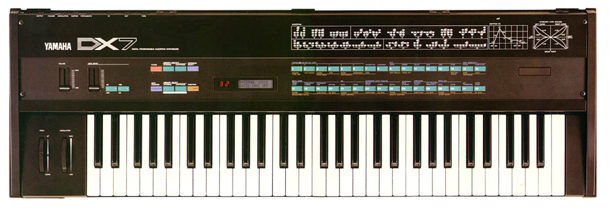
\includegraphics[width=0.95\textwidth]{dx7.png}
\caption{Yamaha DX7}
\label{fig:dx7}
Quelle: \url{http://www.electricdruid.net/images/interface/larger/YamahaDX7.jpg}
\\Stand 09.06.2015
\end{figure}

Durch den großen Erfolg des DX7 konnte Yamaha in den nachfolgenden Jahren viele Weiterentwicklungen auf den Markt bringen. In den Jahren 1983 bis 1989 brachte Yamaha über 20 weitere digitale Synthesizer heraus. Jedoch wurden über die Zeit andere Syntheseverfahren günstiger und für den Markt besser geeignet. Deshalb entwickelte Yamaha 1990 mit dem SY77 Synthesizer ein Gerät, das FM-Synthese und ein anderes digitales Klangsyntheseverfahren namens Sampling in Einem vereinte.\cite{fmGS1}

Ab Mitte der 1990er wurden Personal Computer leistungsfähig genug, um Synthesizer ohne Verzögerung durch eine Midi Tastatur ansprechbar zu machen. Heutzutage findet digitale Audioverarbeitung nahezu ausschließlich softwareseitig statt, weshalb Hardwaresynthesizer wie der DX7 an Bedeutung verloren haben. Speziell dieser wurde jedoch durch die Firma Native Instruments in Form des FM7 in Software nachgebaut. Dessen Weiterentwicklung, der FM8, findet heute noch Verwendung. Auch ist der DX7 heute bei Nostalgikern noch sehr beliebt.\cite{fmGS1}